\subsection{Calibration} 

    The calibration is needed to map each pixel on the CCD to a specific wavelength. Such a map is refered to as a wavelength solution. To do this, we need a light source with known frequencies, preferably many discret peaks. EXPRES uses a Thorium Argon lamp for an initial trial wavelength solution and then a laser frequency comb (LFC) for an more precise solution.
    
    The Thorium Argon lamp produces 4,000 lines across 82 orders, which can be identified and mapped to a wavelength through a \emph{line atlas}. An intial wavelength solution for all pixels is then produced by linear interpolation. (I this project I have not done this calibration).

    % \begin{figure}[!ht]
    %     \centering
    %     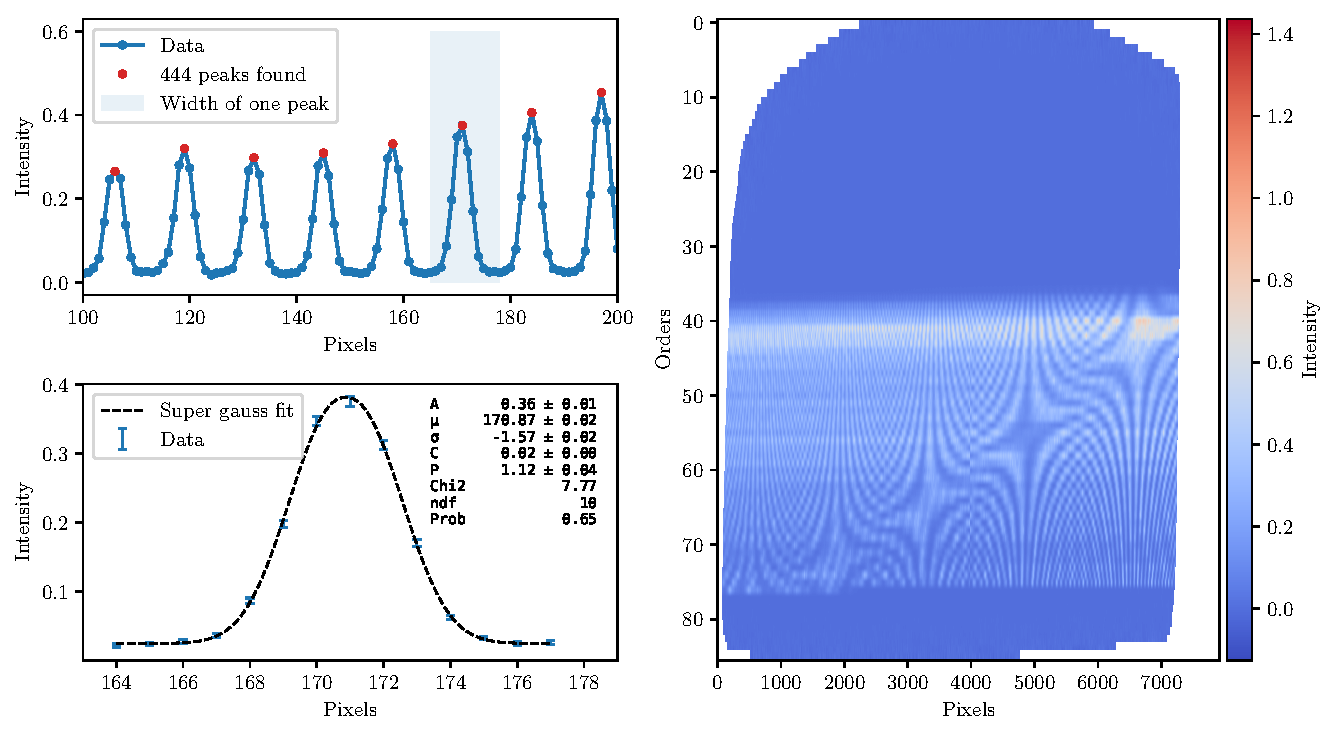
\includegraphics[scale=0.80]{figures/LFC_peak_fitting_overview.pdf}
    %     \caption{Right: Measured intensities for the LFC across the CCD (unitless). Upper left: illustration of a few LFC peaks in order 65. Peaks are identified with scipy peak finder. Lower left: each peak is fitted with a super gauss to find the exact top of the peak with uncertainties.}
    %     \label{fig:LFC_CCD}
    % \end{figure}

    \begin{SCfigure}[1][!ht]%
        \begin{wide}  
            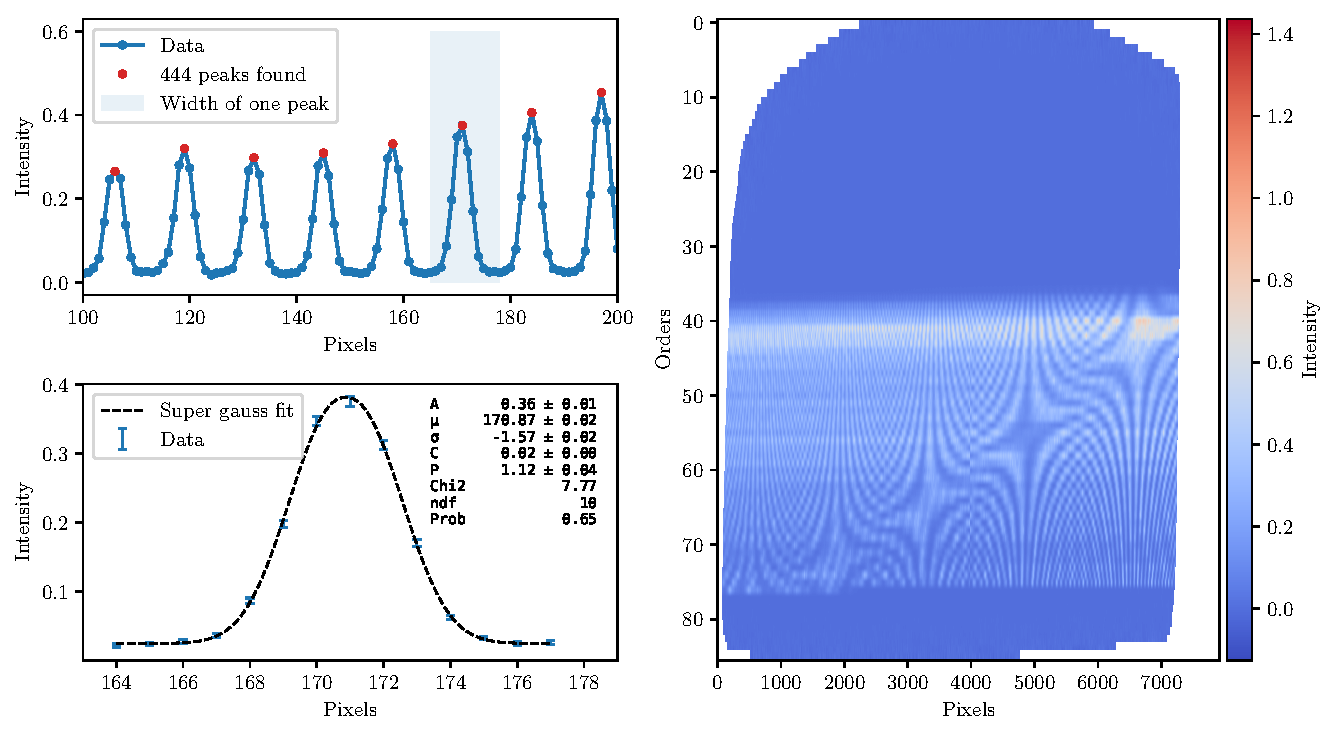
\includegraphics[width=\textwidth]{figures/LFC_peak_fitting_overview.pdf}
            \caption{Right: Measured intensities for the LFC across the CCD (unitless). Upper left: illustration of a few LFC peaks in order 65. Peaks are identified with scipy peak finder. Lower left: each peak is fitted with a super gauss to find the exact top of the peak with uncertainties.}
            \label{fig:LFC_CCD}
        \end{wide}
    \end{SCfigure}
    


    The LFC generates a series of equadistant (evenly spaced) spectral lines, typically 20,000 lines across 50 orders. The range of the LFC is thus shorter, and for this reason the ThAr exposures can also be used for a rough calibration outside the LFC range. The frequencies of the LFC peaks are given by the relation
    
    \begin{equation}
        \label{eq:LFC_freq_eq}
        v_{n}=v_{\text{rep}} \times n+v_{\text{offset}}
    \end{equation}

    for integers $n$. The repetition rate $v_{\text {rep }}$ and offset frequency $v_{\text {offset }}$ are referenced against a GPS-disciplined quartz oscillator, providing calibration stability corresponding to a fractional uncertainty of less than $8 \times 10^{-12}$ for integration times greater than $1 \mathrm{~s}$. (p. 8, \cite{first_RV_from_EXPRES}). The values I have used in the calibration, $v_{\text{rep}} = 14e9$ and $v_{\text{offset}} = 6.19e9$, were provided by Lars Buchhave, but may be outdated. See figure \ref{fig:LFC_CCD} right side for a plot of the intensities measured across the CCD.

    The following procedure is followed to determine the location of the LFC peaks on the CCD: 1) Find peaks using scipy peak finding algorithm 2) make data slices around each peak with the size of the average distance between peaks, 3) using iminuit do a $\chi^2$ minimisation fit to each peak with a super-gauss plus a linear background. See figure \ref{fig:LFC_CCD} left side.

    A super-gauss, defined in eq. (\ref{eq:LFC_super_gauss}), is a regular gaussian but with an extra parameter, here denoted $P$, that allows the top of the gaussian to be flattened. The last two terms here add a linear background and an offset. 
    
    \begin{equation}
        \label{eq:LFC_super_gauss}
        f(x ; A, B, C, P, \mu, \sigma) = A \exp \left(-\left(\frac{\left(x-\mu\right)^{2}}{2 \sigma^{2}}\right)^{P}\right) + B(x-\mu) + C
    \end{equation}

    The fit then is a minimisation of  

    \begin{equation}
        \label{eq:chi2_super_gauss}
        \chi^{2}=\sum_{i=1}^{N}\left[\frac{y_{i}-f(x ; A, B, C, P, \mu, \sigma)}{\sigma_{i}}\right]^{2}
    \end{equation}

    Where $N$ is the number of data points, $x$ is pixel-space, $y_i$ and $\sigma_i$ is the measured photon count and uncertainty respectively. The fit returns the values and uncertainties for the parameters $A, B, C, P, \mu, \sigma$ when the value of $\chi^2$ is minimized.
    
    We are most interested in $\mu$, which gives the position of the LFC peak on the CCD (in pixel-space). With the intial rough wavelength solution dervied from the ThAr lamp (precalculated in the data set that I've used) I can determine what the approximate wavelength of the LFC peak should be. To find the better wavelength solution I then go look up the closest frequency given by eq. \ref{eq:LFC_freq_eq}. And we now have a map of ~20,000 points on the CCD with a good wavelength solution. 
    
    Of course we need to have a wavelength solution for all points on the CCD and to do that I have explored two approaches: cubic interpolation and polynomial fitting. \todoNow{why poly-fit? show plot} I can evaluate the quality of the interpolation calibration by choosing to omit every second peak from the interpolation and then computing the residuals between the omitted peaks and the resulting interpolation function. For the polynomial, I can compute residuals simply by subtracting the location peaks from the fit function. Residuals from the two methods are compared in figure \ref{fig:calib_poly_vs_interp}.

    % \begin{figure}[ht]
    %     \centering
    %     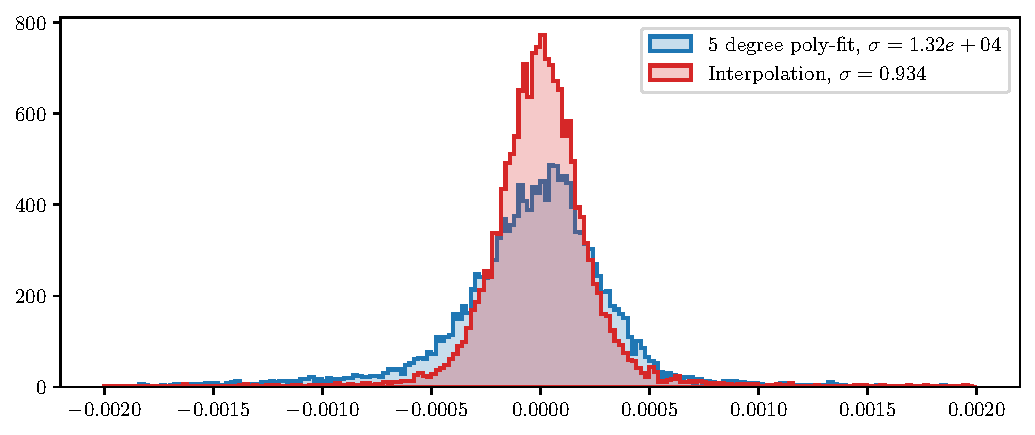
\includegraphics[scale=0.80]{figures/hist_peak_residuals_poly_and_interp.pdf}
    %     \caption{Residuals from calibrations performed through poly-fit and interpolation. Both results contain approximately the same amount of points, but the poly-fit has a much larger spread and therefore appears smaller. \todo{polyfit has 18373 lines, interp has 16888. Why? } Might be because I only use order 40-76 in the interp and all orders with more than 10 peaks for the polyfit. \todoNow{Do new polyfit calib} \todo{find out x units}}
    %     \label{fig:calib_poly_vs_interp}
    % \end{figure}

    \begin{SCfigure}[1][!ht]%
        \begin{wide}  
            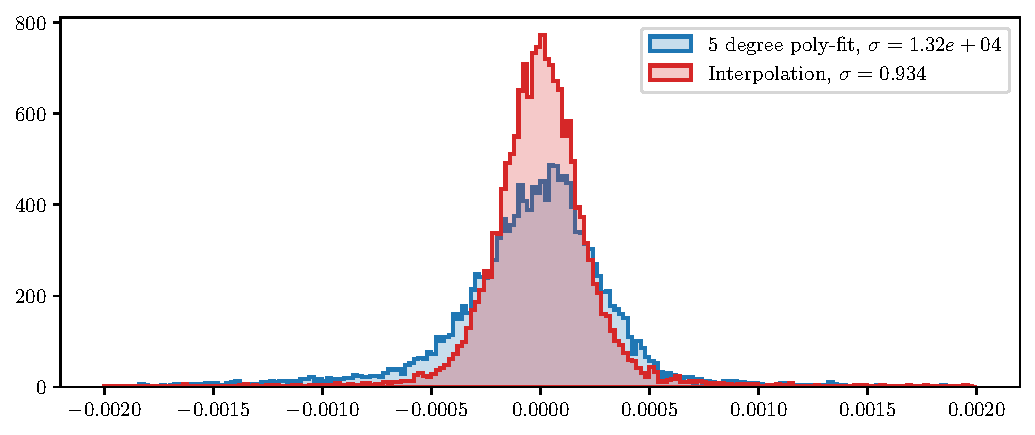
\includegraphics[width=\textwidth]{figures/hist_peak_residuals_poly_and_interp.pdf}
            \caption{Residuals from calibrations performed through poly-fit and interpolation. Both results contain approximately the same amount of points, but the poly-fit has a much larger spread and therefore appears smaller. \todo{polyfit has 18373 lines, interp has 16888. Why? } Might be because I only use order 40-76 in the interp and all orders with more than 10 peaks for the polyfit. \todoNow{Do new polyfit calib} \todo{find out x units}}
            \label{fig:calib_poly_vs_interp}
        \end{wide}
    \end{SCfigure}

    The standard deviation of the residuals from the interpolation come out much smaller than that of the polyfit (values specified in figure \ref{fig:calib_poly_vs_interp}), in this example, suggesting that the interpolation method is superior. It is also worth noting that because the interpolation was done on only half the data points, it will be even better when performed on all data points. A similar comparison was done to determine that the polynomial fit got better with increasing degrees until 5th. \todo{specify what file?}

    \vspace{0.5cm}

    \todo{add graph comparing residuals using gauss vs super gauss}

    \todo{perhaps add plot of changes in parameters across the CCD}

    \todo{specify run times for calibration using poly fit and interp}

    \subsubsection{Errors in the calibration data}

    The LFC fits files come with an uncertatiny on the photon count (spectrum). It appears however that this uncertatiny might be a bit underestimated. We can see this by plotting the $\chi^2$- and P-values for the LFC peak super-gauss fits, as done in figure \ref{fig:calib_errors}. The $\chi^2$ value should be roughly equal to the number of degrees of freedom in the fit, which is: 

    \begin{equation}
        \label{eq:ndof}
        N_\text{dof} = N_\text{data-points} - N_\text{fit-parameters} =  13 - 5 = 8.
    \end{equation}

    The number of data points per fit I set to be the rounded average distance bewteen peaks in a given order. Although the LFC should generate equadistant peaks, this does vary bewteen 13 and 18 points as we go through orders, most fits having 13 data points (see figure \ref{fig:N_data_points} in appendix \ref{appendix:LFC_errors}). We should therefore see a spike in the $\chi^2$ values roughly around 8, falling of at a slower pace to the right side. Looking again at figure \ref{fig:calib_errors}, this is not the case for the errors as provided (scale-factor 1). But multiplying by $\sqrt{3}$ we get much closer. $\sqrt{10}$ is overdoing it, however. I looked at several other scaling factors bewteen $\sqrt{3}$ and $\sqrt{10}$, see figure \ref{fig:calib_errors_extensive} in appendix \ref{appendix:LFC_errors} for details, and $\sqrt{3}$ comes closest to giving a peak at 8.
    
    Another check is that the probability distribution should be roughly flat. \todo{explain why, \href{https://stats.stackexchange.com/a/481843/353364}{help}}.
    
    \begin{SCfigure}[1][!ht]%
        \begin{wide}  
            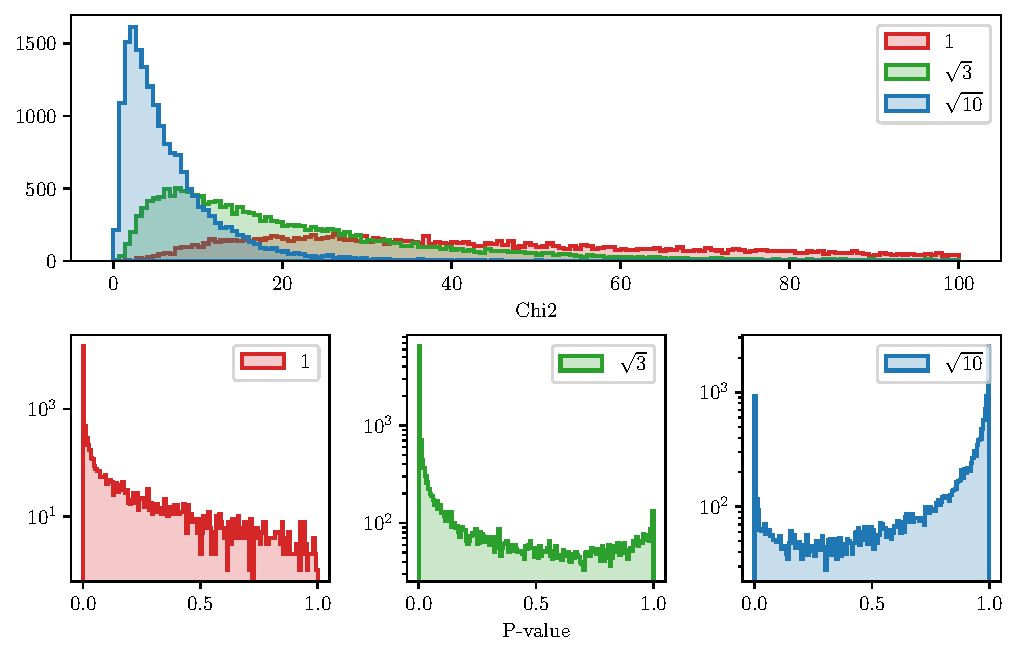
\includegraphics[width=\textwidth]{figures/calib_errors2.pdf}
            \caption{Chi2-values and P-values from individual LFC peak super-gauss fits with photon count (spectrum) errors multiplied by different scale-factors (1, $\sqrt{3}$ and $\sqrt{10}$). See text for more datails.}
        \label{fig:calib_errors}
        \end{wide}
    \end{SCfigure}
    

    \todo{explain why we use factors of square-root:} Something to do with putting into the chi2 which is a square sum, so the square-root goes away. 

    \bigbreak

    \noindent \textbf{Effects on calibration:} \newline
    The errors used during the production of the calibration residuals shown in figure \ref{fig:calib_poly_vs_interp} I have already multiplied by $\sqrt{3}$. This gaves us a $\sigma = 0.934$, without this correction I got $\sigma = 2.34$. 

    \todo{Computing the sigma for different error scaling factors gave very jumpy results.. why?} 

\subsection{RV extraction}

    \todoSmall{mention that so far I am using pre-calibrated data, because we are missing the right data}
    
    % \marginpar{
    %     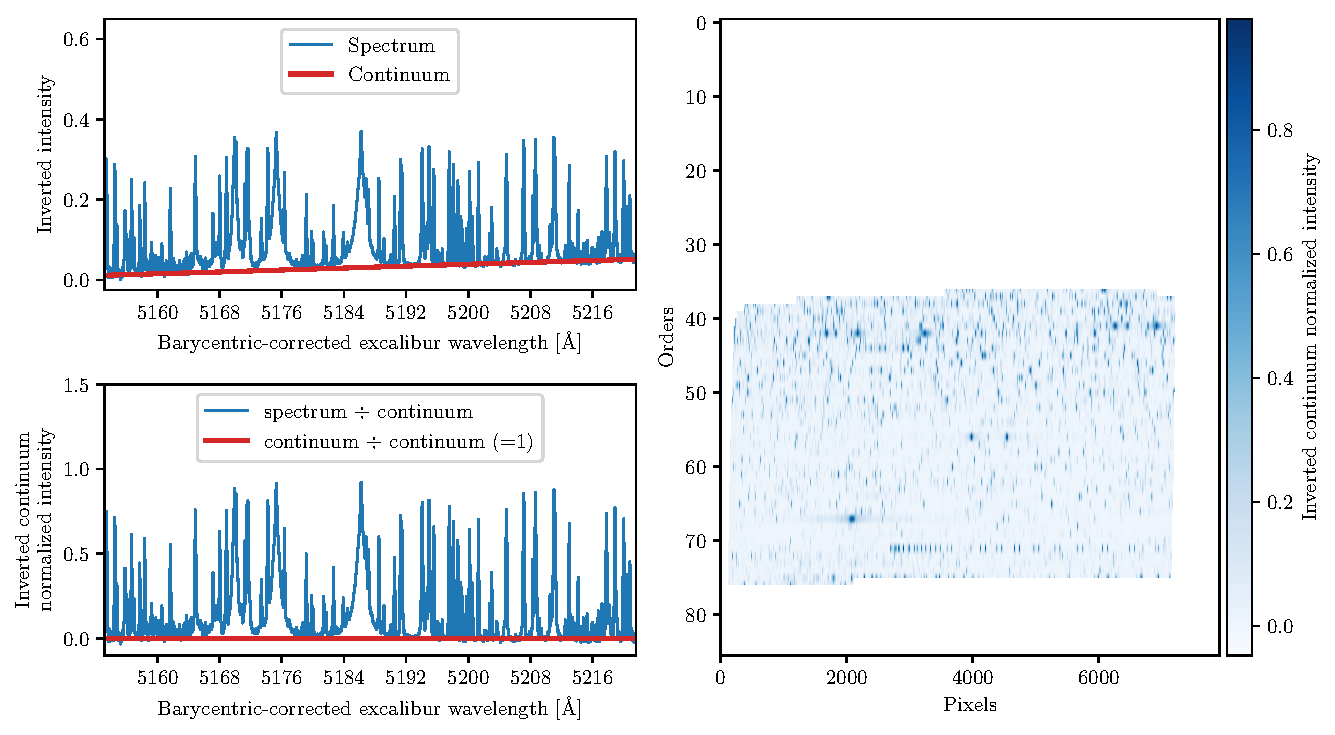
\includegraphics[width=0.95\marginparwidth]{figures/rv_data_overview.pdf}
    %     \captionof{figure}{Carl Friedrich Gauss, født 1777, er bedst kendt for normalfordelingen}
    % }

    In signal processing, cross-correlation is a measure of similarity of two series as a function 
    of the displacement of one relative to the other.

    To extract radial velocity we need to measure the doppler shift between spectras from different days of observation. The most straight-forward way to do this is to compute the cross-correlation, since, in signal processing in general, the cross-correlation is exactly a measure of the similarity of two data series as a function of the displacement of one relative to the other.

    Due to a lack of access to data consiting of star spectra with associated LFC captures, I've worked on RV extractions using already calibrated data provided by Lily Zhao. This data has been calibrated using a technique called excalibur \cite{zhao2021excalibur}.

    In this project I've worked with data provided by Lily Zhao, specifically for the star HD 34411. This data is already LFC calibrated using a technique called Excalibur. Top left of figure \ref*{fig:rv_data_overview} shows an extract of wavelength vs. intensity data from an observation of HD 34411. The file also includes a model of the continuum function, with which we can normalize the spectrum through division, shown bottom left. On the right side is plotted all normalized data within the EXCALIBUR mask, i.e. data marked as having a proper calibration. 

    \begin{SCfigure}[1][!ht]%
        \begin{wide}  
            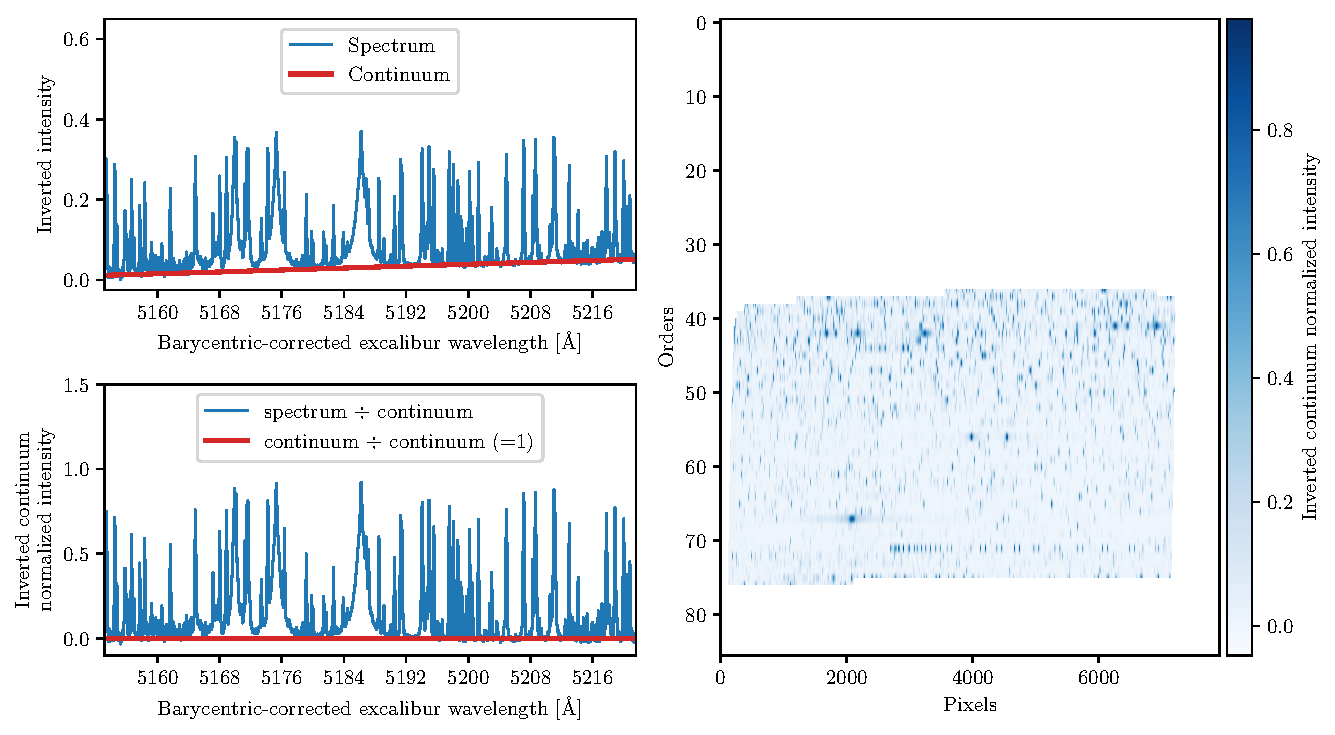
\includegraphics[width=\textwidth]{figures/rv_data_overview.pdf}
            \caption{Overview of excalibur calibrated data from an observation of HD 34411. Upper left: extract of wavelength solution vs. intensity. Lower left: continuum normalized spectrum. Right: all continuum normalized data within the excalibur mask.}
            \label{fig:rv_data_overview}
        \end{wide}
    \end{SCfigure}
            
    To perform a smooth minimization of a shift parameter, it is however necessary to have continuous data, so the first step is to perform a cubic interpolation of the spectra data. In practice I do this inside my chi2 minimization function. Taking the spectra data and wavelength solution from two different observations, but multiplying one of the wavelength with the doppler shift factor from eq \ref{eq:our_doppler}before performing the interpolation. The interpolation functions are then evaluated in the range of wavelength solutions common to both observations, using $N=1000$ steps.\footnote{1000 steps was chosen as the best balance between run time and resulting uncertainty. See figure \ref{fig:err_vs_run_time} in appendix \ref{appendix:RV_extraction}. \todo{Are errors correct?}} 
    
    \begin{equation}
        \label{eq:shift_fit_chi2}
        \chi^{2}=\sum_{i=1}^{N}\left[\frac{y_{i}-f(x; A)}{\sigma_{i}}\right]^{2}
    \end{equation}
    
    where $y_i$ are the unshifted interpolated photon counts for one file and the function $f(x; A)$ is an cubic interpolation function given my the intensity values of the second observation with wavelength values shifted by equation \ref*{eq:our_doppler}, then evaluated on the common wavelength range:
    
    \begin{equation}
        f(x; A) = \textbf{interp}[x \times ( 1 + A/c), y]\,(x_\text{common})
    \end{equation}

    The errors, $\sigma_i$, are also computed through interpolation.\footnote{The errors, $\sigma_i$, which of course also need to be continuous, are computed by: 1) computing another two cubic interpolations for the non-shifted observation, one with photon counts \emph{plus} photon count errors and another one with photon counts \emph{minus} photon count errors. Both interpolations are then evaluted on the same common wavelength range with $1000$ steps. The error for each data point is then computed as the mean difference between the measured value and the upper and lower error.}
    
    I then compute the cross-correlation and obtain the wavelength shift as a minimization of eq (\ref{eq:shift_fit_chi2}) using iminuit. When it comes to choosing data for fitting there is some freedom. I've explored 2 options: 1) fitting order by order and 2) fiting feature by feature, i.e. locating and individual peaks in the spectra, fitting features obvisouly being the more complicated approach. 
    
    \bigbreak
    \noindent\textbf{Finding and matching features across observations}
    
    \todo{}

    \bigbreak
    \noindent\textbf{Extracting relative shifts from over constrained system - matrix reduction:}
    
    The end desired end result is a plot of the relative radial velocities as a function of time or observation. If we were to simply compare each observation with the following one, our results would become correlated in the sense that the difference between day 1 and day 10, let's say, will depend on the quality of all observations in between. To circumvent this, we can compute the relative shift between all observations, yielding an $N\times N$ upper triangular matrix, where each cell is the shift bewteen observations $i$ and $j$, and thus with a diagonal of 0. I will call this matrix $\Delta V_r^{ij}$, see figure \ref*{fig:shift_matrix}, here non-barycentric-corrected data is used for the sake of illustration. 
    
    \begin{SCfigure}[1][!ht]%
        \begin{wide}  
            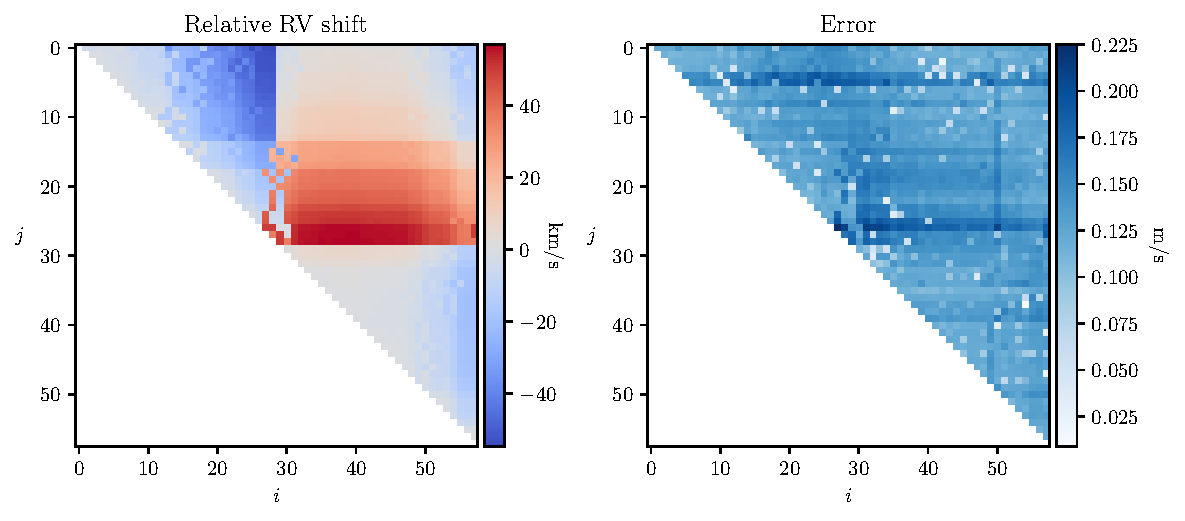
\includegraphics[width=\textwidth]{figures/shfits_matrix_non_bary.pdf}
            \caption{Wavelength shift matrix computed for data from HD 34411. The data emplyed is from the "wavelength" column in the fits file, meaning it is not bary-centric corrected, nor excalibur calibrated. Each cell shows the median relative radial velocity between feature $i$ and $j$. The diagonal should be zero and has been ommited for the sake of computational speed.}
        \label{fig:shift_matrix}
        \end{wide}
    \end{SCfigure}
            
    The following chi2 minimization with the fit parameters $V_r^i$ (an array of length $N$) will then find a list of values that best describe the whole matrix. In other words, it finds the relative shift for each observation with all other observations. 

    \begin{equation}
        \label{eq:matrix_reduction_fit}
        \chi^{2}=\sum_{i,j = 0}^{N}\left[\frac{ \Delta V_{r}^{ij} - (V_r^i - V_r^j) }{\sigma(\Delta V_{r}^{ij})}\right]^{2} \quad : \quad i < j.
    \end{equation}
    
    The resulting fit parameters are plotted in figure \ref{fig:shift_non_bary_centric}, and we see a clear signal of the Earth movement around the barycenter of the solar system. Considering the resulting chi2- and p-value, it is possible that my errors are much too small. But I do get a wavelength/period close to that of one Earth year.

    \begin{SCfigure}[1][!ht]%
        \begin{wide}  
            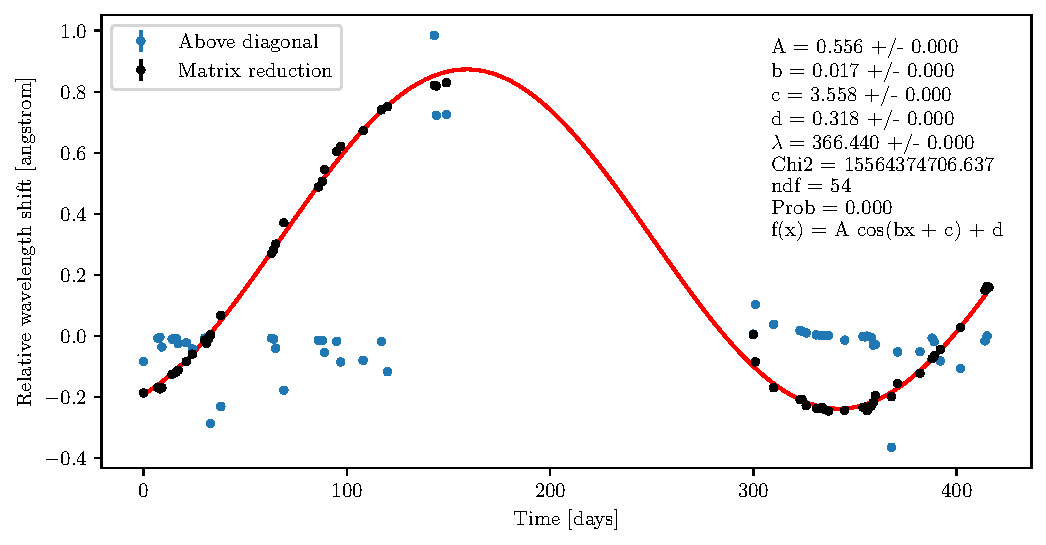
\includegraphics[width=\textwidth]{figures/shift_non_bary_centric.pdf}
            \caption{Computed relative wavelength shifts for HD34411 using non-calibrated, non-bary-centric-corrected data (column = "wavelength"). Blue: the shifts from day to day. Black: values computed through the chi2 minimization.}
            \label{fig:shift_non_bary_centric}
        \end{wide}
    \end{SCfigure}
    
    But of course we would like to have radial velocities, which allow us to determine the minimum mass of the planet.
    Converting to radial velocity turns out to be more complicated than expected, as there is no direct conversion factor, but it depends on the specific wavelenght. In general a (non-relativistic) shift in velocity from a shift in wavelength is given by

    \begin{equation}
        \label{eq:delta_velocity}
        \Delta v = \frac{\lambda_1 - \lambda_0}{\lambda_0} \times c.
    \end{equation}

    But as mentioned for this we not just the shift but also the actual position of each of the peaks. 

    \todo{} So I need to do gauss fits (?) for the features and find the exact location. Perhaps compute the RMS per line, like they do in eq 5 of excalibur paper:

    $$
        \mathrm{RMS} / \text { line }\left[\mathrm{m} \mathrm{s}^{-1}\right]=\sqrt{\sum_{n=1}^{N} \sum_{p=1}^{P} \frac{\left[\frac{\left(\lambda_{n, p, \text { pred. }}-\lambda_{p, \text { theory }}\right)}{\lambda_{p, \text { theory }}} \times c\right]^{2}}{N \times P}}
    $$

    \todo{add run times}



